\documentclass[conference]{IEEEtran}

\usepackage{bm}
\usepackage{amsmath}
\usepackage{graphicx}
\usepackage[colorlinks=true,urlcolor=blue]{hyperref}
\usepackage{geometry}
\geometry{margin=1in}
\usepackage{multicol}
\usepackage{paralist}
\usepackage{todonotes}
\setlength{\marginparwidth}{2.15cm}
\usepackage{booktabs}
\usepackage{enumitem}


\begin{document}
%
% paper title
% can use linebreaks \\ within to get better formatting as desired
\title{Midway Report}


% author names and affiliations
% use a multiple column layout for up to three different
% affiliations
\author{\IEEEauthorblockN{Xiaoqiu Huang}
\IEEEauthorblockA{School of Computer Science\\
Carnegie Mellon University\\
Email: xiaoqiuh@andrew.cmu.edu}}
% make the title area
\maketitle

% For peer review papers, you can put extra information on the cover
% page as needed:
% \ifCLASSOPTIONpeerreview
% \begin{center} \bfseries EDICS Category: 3-BBND \end{center}
% \fi
%
% For peerreview papers, this IEEEtran command inserts a page break and
% creates the second title. It will be ignored for other modes.
\IEEEpeerreviewmaketitle



\section{Introduction}
Usually, many shallow-strutured achitectures, such as kernel perceptron, logistic regression, SVM and so on, are utilized in natural language processing. Due to the high efficiency and good performance, they are still very popular in NLP field. However, these algorithms with simple models and limited represention power cannot achieve impressing results in dealing with more complicated tasks. In order to extract more complex features and better represent human language, multiple layers models or deep structure models are designed to handle more  complicated human language problems.

The purpose of deep learning is to extract more features from human languages through adopting neural networks with deep structure. So the idea of deep learning originates from artificial neural network(ANN).The combination of feed-forward neural network and back propagation(BP) algorithm\cite{rumelhart1988learning} make the neural network a good model for learning the representation of natural language. (works concerning NN and NLP). However, BP has many shortcomings which limit its ability in learning features. The most important is that as the number of layers becomes large, it is hard for BP to propagate the error from hidden layers to input layers. In another words, BP algorithm is a optimization method based on optimal local search and easy to achieve local optimum as the structure becomes deep.

However, the algorithm of deep learning can not only adopt deep struture but also achieve better optimization results. In 2006,  a fast learning algorithm for deep belief nets(DBN) was proposed by Hinton et al.\cite{hinton2006fast}. Instead of using BP algorithm to optimize all of weights in each layers, a greedy learning algorithm was adopted to train the model layer by layer. But since learning one layer at a time is not optimal, a wake-sleep algorithm was utilized to fine-tune the weights of neural network. In the 2007,  another paper proposed a unsupervised deep neural network model\cite{bengio2007greedy}. In this model, each layer is trained an auto-encoder. As the idea become popular, many different deep structures are adopted in deep neural networks, such as recursive neural network, recurrent neural network and so on.

\section{Introduction to the structure of deep learning}
\subsection{Neural language model}
In traditional NLP model, the input of the classifer is just one-hot features or TF-IDF features of text. However, this model suffers from the curse of dimensionality. When the number of documents in the corpus becomes large, the matrix of features will become sparse. Therefore, Bengio et al.\cite{Bengio2003NLP} proposed a new neural language model which generates distributed representations for each word in the corpus. That means each word in the documents has a fixed length of feature vector. With the feature vectors of each term, we can measure the similarity between different words or generate the vector representation of each document.

In our model, each word will be first transformed to word vector by the tool named word2vec\cite{mikolov2013efficient}. The tool will first train the neural language model on our data set and then generate the word vector of each term.

\subsection{Recursive Autoencoder}
Autoencoder is a neural network model that learns the function $f(x)=x$ in order to learn the reduced representation of the input text. As we can see in the figure 1, autoencoder is only a three-layer neural network. We want to utilize the hidden layer to generate the similar vector as the input vector. And after traning the model, the hidden layer can be treated as the condensed feature of the input vectors. Therefore, the training objective is to minimize the distance which is known as reconstruction error between the input and the output of NN. When applying such structure into our model, the input of the autoencoder is word vectors of two terms. After traning the model, the vector of hidden layer can be seen as the condensed feature of these two words.

\begin{figure}[ht]
\centering
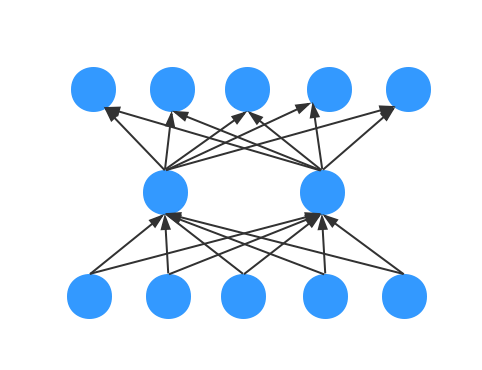
\includegraphics[width = 0.8\linewidth]{figure/autoencoder}
\caption{Autoencoder}
\label{fig:ae}
\end{figure}

However, only using the structure of autoencoder may not effectively model the text. If we set the input of autoencoder as the vectors of all terms in one document and try to generate the condensed features of the document, there will be so many parameters to optimize and the structure of the text is not utilized. In order to solve the problem, the structure of recursive autoencoder was proposed to model the hierarchical structure. Figure 2 shows the structure of recursive autoencoder.
\begin{figure}[ht]
\centering
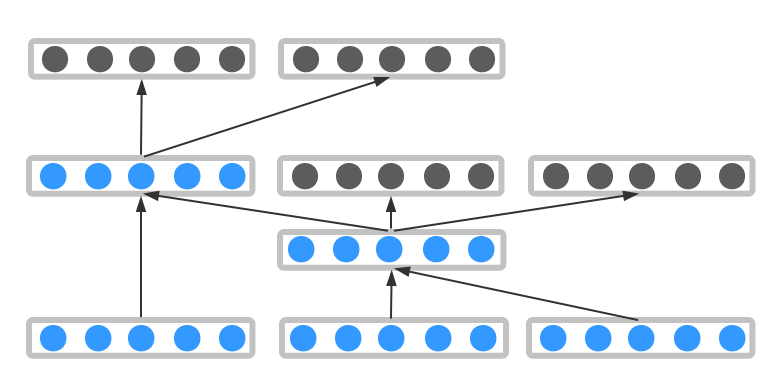
\includegraphics[width = 1.0\linewidth]{figure/recursiveautoencoder}
\caption{Recursive Autoencoder}
\label{fig:rae}
\end{figure}


In each layer, several terms are combined to generate the condensed features which will be utilized as the input of the next layer. At the final layer of recursive autoencoder, the vector of hidden layer will be the vector representation of the whole documents.

One of the key problem in such structure is how to combine different terms. There are mainly two ways. One way is to adopt the grammer tree which generated in advance. Each word will be combined in the same way as they are merge in the grammer tree. Another way is to utilize the greedy algorithm. At each layer, each pair of the adjacent words will be first combined and output reconstruction error. Then the pair of words with smallest error will be first combined. Using this greedy algorithm, the vector of each document can also be generated. In the experimental part, the effectiveness of the two structured will be compared.

\subsection{Semi-supervised Recursive Autoencoder}
In the traditional recursive autoencoder model, the network is trained only by the document itself. Therefore, it is the unsupervised model. In certain scenario, the label information of documents can be incorporated into the model and turn the model into a semi-supervised model.

One of the semi-superivised recursive autoencoder model has been proposed by socher et al.\cite{socher2011semi} in order to handle the issue of sentiment analysis. The structure of recursive autoencoder is presented as follows:
\begin{figure}[ht]
\centering
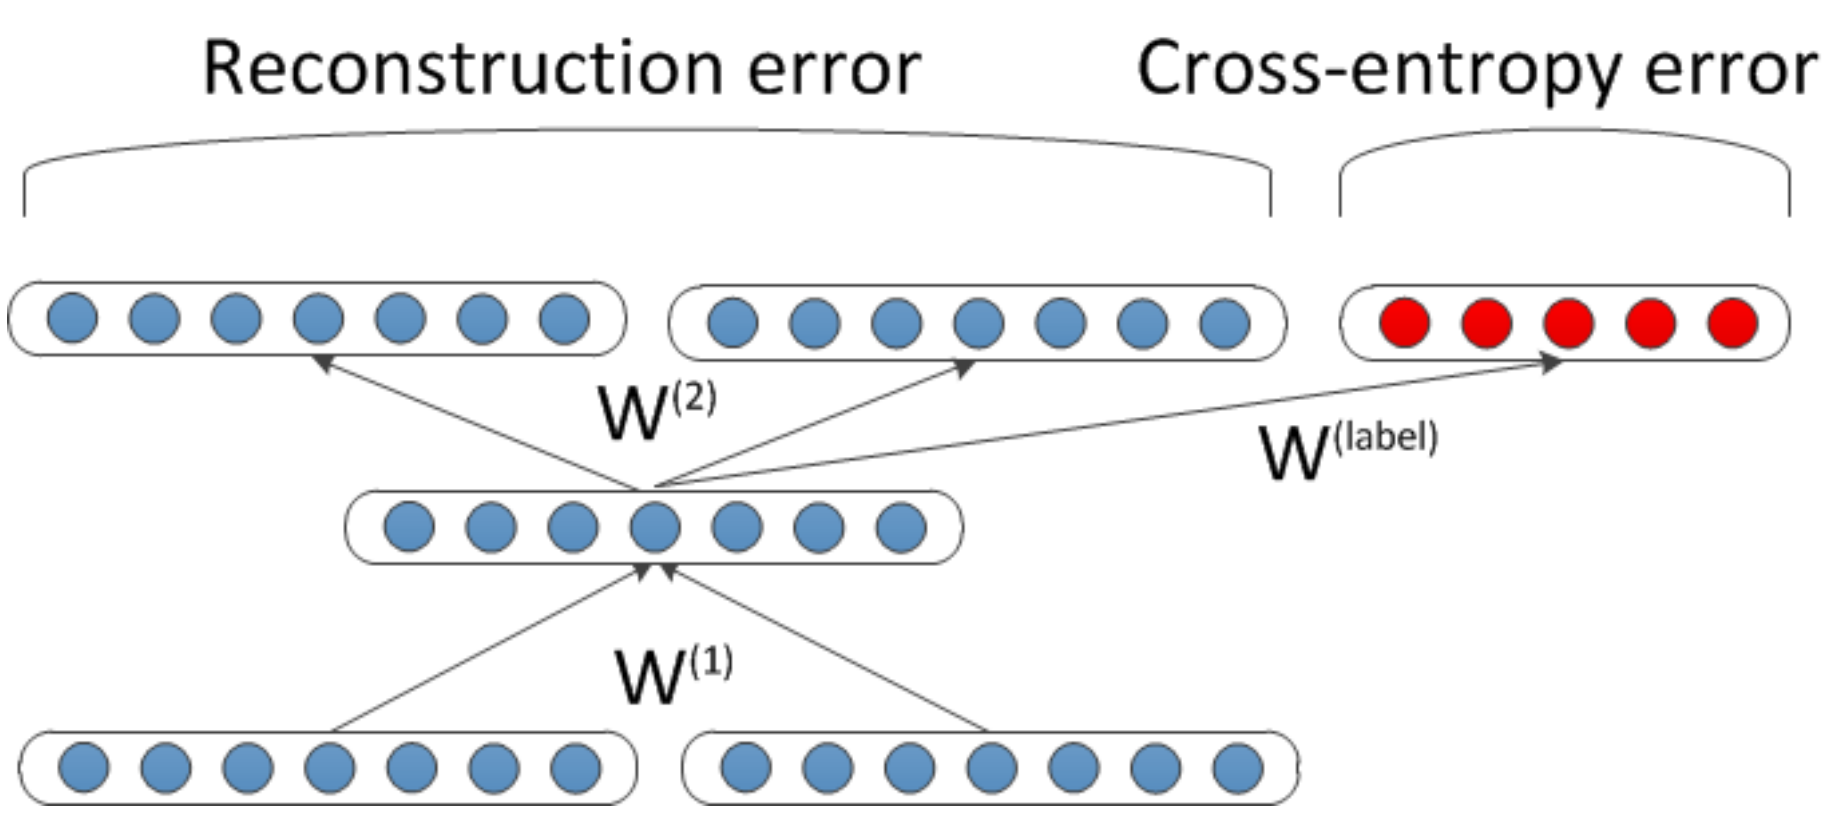
\includegraphics[width = 1.0\linewidth]{figure/semiautoencoder}
\caption{Semi-supervised Autoencoder}
\label{fig:sae}
\end{figure}

As we can see from the figure, the input of the model is also the distributed representation. After being processed by the hidden layer, the output layer reconstructs the input vector. In order to measure the performance of the representation, the reconstruction error is computed as the distance between the input vector and output vector. Also we can assign different terms with different weights. So
\begin{equation}
\begin{split}
 & E_{rec}([c_{1};c_{2}];\theta) \\
 & = \frac{n_{1}}{n_{1}+n_{2}} ||c_{1}-c_{1}'||^2 + \frac{n_{2}}{n_{1}+n_{2}} ||c_{2}-c_{2}'||^2\\
 \end{split}
\end{equation}
, where n denote the number of words. In addition, c denotes the vector of input and c' present the vector of output.

Also, in order to predict the sentiment of the sentence, an extra output unit is added to generate the sentiment label. And this generated label will be compared with the correct label. A softmax function is utilized in this scenario to generate the probability of each label. And author use the cross-entropy error to measure the correctness of the model.
\begin{equation}
\begin{split}
 & E_{cE}(p,t;\theta) \\
 & = -\sum_{k=1}^{K}{t_{k}\log{}d_{k}(p;\theta)}\\
 \end{split}
\end{equation}
, where $t_{k}$ denotes the target label and $d_{k}$ denotes the probability of each label.

After combining the two process, we can compute the reconstruction error and cross-entropy error. And the objective is to minimize the weighted sum of the two errors as follows:
\begin{equation}
\begin{split}
 & E([c_{1}; c_{2}]s, ps, t, θ) = \\
 & = \alpha E_{rec}([c_{1}; c_{2}]_{s}; \theta) + (1 - \alpha)E_{cE}(p_{s}, t; \theta).
\\
 \end{split}
\end{equation}

\bibliography{IEEEabrv,bib/dp}
\bibliographystyle{IEEEtran}

% that's all folks
\end{document}


